\chapter{Report's goals}

\section{Introduction}

At the CMS detector, approximately 1.6 terabits per second of data is generated (cite for number). It is, however, neither feasible nor practical to read out all the events. To overcome this, the CMS data acquisition system runs a two level trigger system to reduce the data throughput: the Level-1 Trigger (L1T) and the High-Level Trigger (HLT). For the expected High-Luminosity LHC (HL-LHC) upgrade, changes to the trigger system are anticipated (CMS-TDR-021 and CMS-TDR-022, to be properly cited) to handle the new experimental conditions, which result in higher pile-up (PU) and increased data complexity (PU cite). 
\newline \newline 
The main constraint to the current offline reconstruction quality and quantity at CMS is encountered in form of the processing capacity of Tier-0. Once an event is accepted by both L1T and HLT, it is processed and fully reconstructed at Tier-0. The output rate is furthermore limited by the output bandwidth. These constraints impose substantial restrictions on the number of events that can ultimately be processed and stored for offline physics analysis. The consequences of this is that certain phase space regions remain unexplored by the CMS collaboration (exclusion plots). It is thus crucial to rethink our data acquisition strategy, which in turn will aid in future new physics searches. The Nest Generation Trigger (NGT) project at CMS aims to supplement the planned upgrades, further enhancing the physics potential of CMS during the high-luminosity era. The overarching goal is being able to fully reconstruct a larger data rate in real-time.
\newline \newline
To achieve this goal, a novel calibration workflow is needed, which the 3.4 Optimal Calibration task is dedicated to. The main objective of this task is to design a fast calibration workflow that meets or exceeds the resolution Tier-0 provides in the offline reconstruction, while automating and optimizing the calibration processes. This will also introduce data buffering at the HLT and a prototype of this workflow is planned to be deployed within a year. As a first step, task members acquainted themselves with the existing calibration workflows and selected ideal candidates for the prototype, thanks to an collaboration-internal survey. In this report, we will present the current calibration workflow(s) at CMS, discuss the identified candidates and integration of our workflow into the DAQ system and finally provide a conclusion and outlook from the first year of the 3.4 Optimal Calibration Task.

\section{CMS Calibration Workflows}

%%% Some introductory text to explain the main concepts.

\section{CMS Calibration Workflows}
The CMS detector is composed of various sub-detectors, each with specific tasks and functionalities. This makes data acquisition a highly intricate task.

Fully reconstructing events measured by the detector requires precise knowledge of the detector conditions at the time of data taking. Numerous factors are to be considered frequently: What is the energy response of a given scintillator in the calorimeters? What are the efficiencies of individual pixels within the tracker? Is everything still exactly located where it was initially placed? What is the exact position of the proton-proton collision? Which detector components do not deliver the desired efficiency anymore? To consistently address these issues, a calibration and alignment (AlCa) workflow has been put in place to tackle the various challenges. The workflow provides direct feedback to the reconstruction algorithms to ensure full quality for the data taken. The frequency of condition updates ranges from seconds to moths. There are currently 326 conditions (records/tags) in the latest HLT Global Tag (\texttt{140X\_dataRun3\_HLT\_v3}) used during LHC Run 3 p-p data taking in 2024. 
\newline \newline
Central to the AlCa workflow is the \textbf{Prompt Calibration Loop} (PCL), where conditions are derived prior to full reconstruction. After the HLT, there are two main reconstruction streams: \textit{express} and \textit{physics}. The express stream processes a subset of the triggered data and runs the express reconstruction. The express stream has highest priority at Tier-0 and is completed within 1-2 hours. The conditions are derived from this stream and uploaded to the offline conditions database (DB). The physics stream then performs the prompt reconstruction, where it uses the conditions from the DB. This is done within 48 hours and the outcome gets stored and then used for physics analysis. These workflows are nicely visualized within Fig. \ref{fig:PCL}. Other calibration workflows exist, such as \textbf{Online to Offline} (O2O). O2O plays a critical role, as it passes on the online conditions within the sub-detector infrastructure to DB, making it accessible for event reconstruction.
\newline \newline

% TODO: General introduction

% TODO: explain general AlCa: calibration vs condition, records, tags, etc.

% Latest GTs:

% NOTE: Introduce prompt/offline in a similar manner?

\subsection{PCL}

\begin{figure}[h!]	
\centering
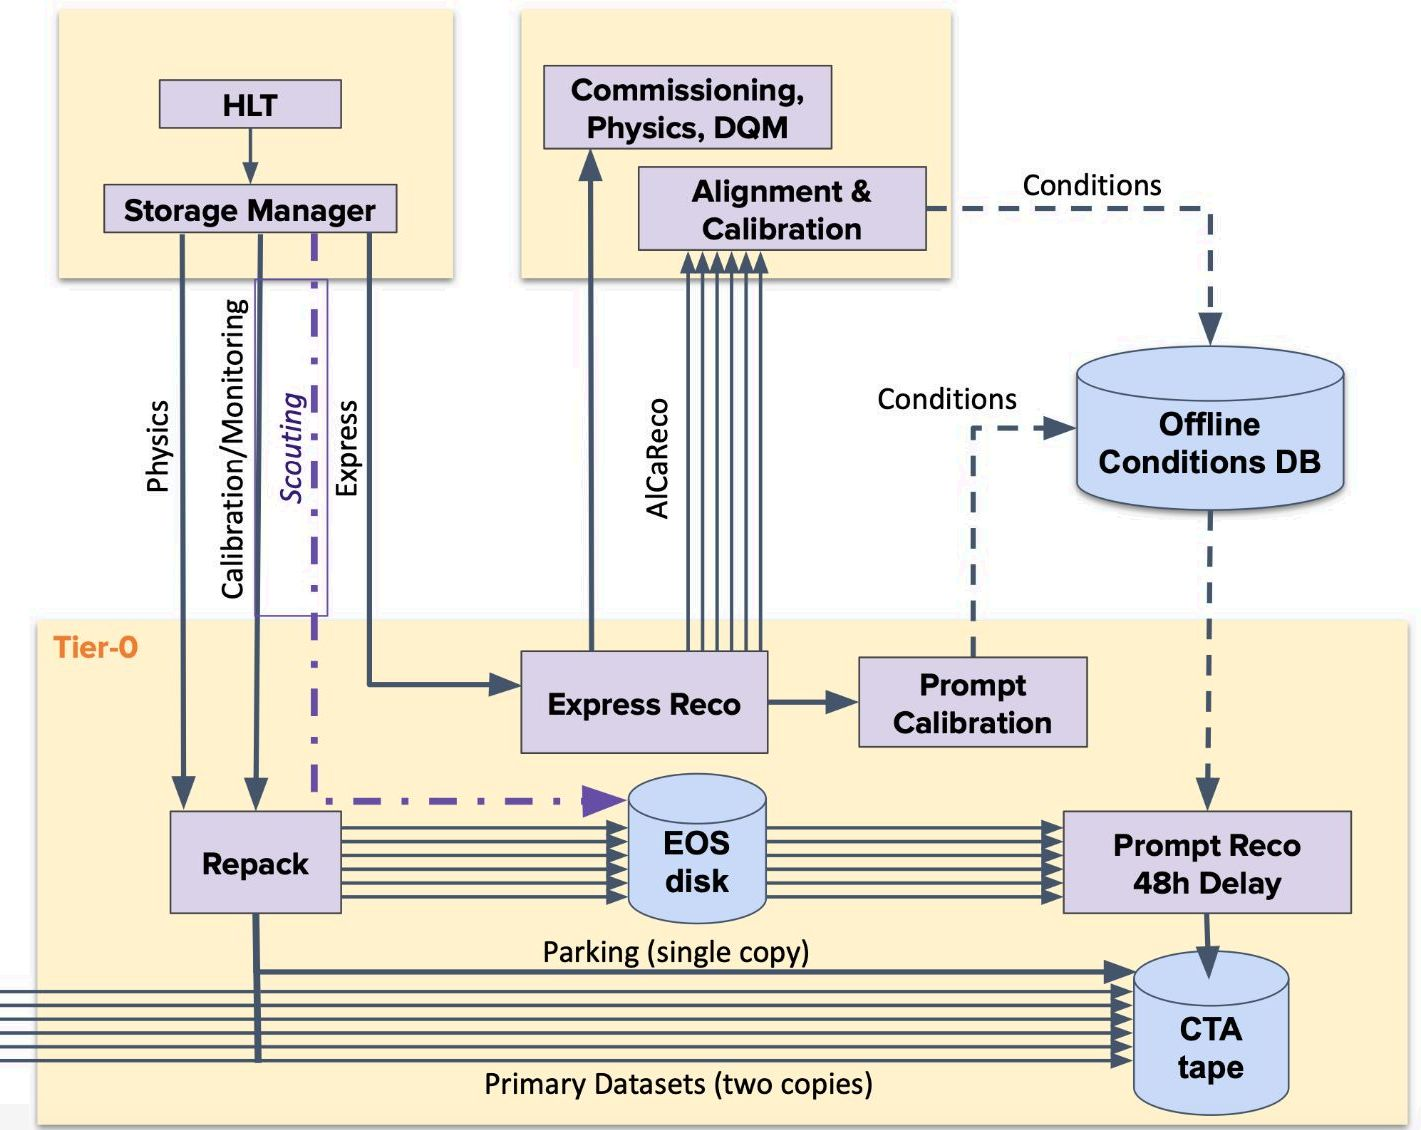
\includegraphics[width=\textwidth]{figures/PCL.jpg} %\hfill
\caption{A schematic overview of the current Prompt Calibration Loop (PCL) implemented at CMS, showcasing its integral role to the data reconstruction workflow. Source for this?}
\label{fig:PCL}
\end{figure}

\subsection{O2O}
\subsection{Other}

%%% Here we should add something about the automation framework






















































% The objective of \ngt{}'s \task{3.1.1} is to reconstruct all events received
% from the L1T at a rate of \SI{750}{\kilo\hertz} during Run-\num{5} data taking,
% eventually with an \emph{Offline-like} quality reconstruction. The
% reconstruction should enable some ``quick and dirty'' analyses using the
% reconstructed objects, without requiring additional steps. In order to
% understand where we are in terms of computing and physics performance, we
% decided to conduct a series of measurements using different scenarios, as
% explined in \ref{sec:measurements}. Considering a
% fixed budget for the farm in Run-\num{4} and Run-\num{5}, we need to determine
% the speed-up factor needed to be able to process the whole L1TA input rate with
% the required quality.
% 
% \section{Measurements}
% \label{sec:measurements}
% 
% As part of the first-year milestones, \task{3.1.1} is responsible for
% delivering a report on the performance of online reconstruction. This report
% will address identified bottlenecks, propose targeted improvements, and outline
% the necessary features for the generic CMS Structure of Arrays (\soa{}). To
% achieve this, we have begun conducting measurements using recent \CMSSW*{}
% releases. Our focus is on three specific performance metrics:
% 
% \begin{itemize}
% \item
%   \textbf{Measure the current performance of the \emph{simplified HLT Phase2
%     menu} for HL-LHC}: This will evaluate the present performance in terms of
%     computing speed and memory usage, with an aim to extrapolate these metrics
%     to 2030, the expected start of HL-LHC operations, and further down to 2032,
%     the beginning of Run-\num{5} operations. This will be done using both a
%     sample of \emph{TTbar} simulated events from the \textbf{Spring24} ongoing
%     campaign under 200PU conditions (and 140PU, if available), and a
%     specifically created \textit{skim} of L1 accepted events over an input
%     sample of \textit{MinimumBias} events, at 200PU.
% \item
%   \textbf{Assess the current performance of the \emph{offline Phase2
%     reconstruction}}: This will be done using both a sample of \emph{TTbar}
%     simulated events from the \textbf{Spring24} ongoing campaign under 200PU
%     conditions (and 140PU, if available), and a specifically created
%     \textit{skim} of L1 accepted events over an input sample of
%     \textit{MinimumBias} events, at 200PU. We will then project this
%     performance to 203{0,2}, considering anticipated improvements in CHF/HS06
%     and the likely shift of some algorithms and reconstruction processes to
%     accelerators. This analysis will help identify the necessary speedup factor
%     required to handle the full L1A rate directly during HLT processing using
%     an \textbf{offline-like reconstruction}, which is the final goal of this
%     task.
% \item
%   \textbf{Account for ongoing development in the \emph{offline Phase2
%   reconstruction}}: Since it is still evolving and lacks some
%   improvements present in the \emph{Run-3 reconstruction}, we also plan
%   to measure the performance of the \emph{Run-3 reconstruction} on a
%     simulated \textit{TTbar} sample with roughly 60PU. We will then identify which
%   modules from the \emph{Run-3 scenario} are missing in the
%   \emph{offline Phase2} sequence, estimate their
%   significance---particularly regarding CPU usage---extrapolate this
%   data to 200PU conditions, and incorporate it into our previous
%   performance measurements.
% \end{itemize}
% 
% All measurements have been done using \CMSSW[14][2][0][1]{}. A few additional patches have been necessary in order to correctly re-process the events. The patches fixed genuine bugs in the Phase\num{2} HLT Menu that were discovered while performing these measurements. Those patches have been submitted upstream to the main \CMSSW*{} release as pull requests (\href{https://github.com/cms-sw/cmssw/pull/46019}{46019} and \href{https://github.com/cms-sw/cmssw/pull/46054}{46054}) and integrated.
% 
% All samples used have been specifically produced to optimize the performance of the Phase\num{2} HLT reconstruction and of the offline reconstruction. Detailed instructions on how to create the samples and about their specificities are avaialble at \href{https://cms-ngt-hlt.docs.cern.ch/Task311/2024/Recipes/}{this link}\cite{ngt-recipes}.
% 
% Once all measurements are completed and the data is available, we will
% be in a better position to propose the next steps for development.
% Specifically, we will understand the extent of \textit{disruption} required to
% meet the highly ambitious goals outlined in this task.
% 
% \subsection{Pie resources}
% \label{subsec:pie-resources}
% 
% All pie-chart resources are usually available at
% \href{https://rovere.web.cern.ch/rovere/Phase2_HLT/circles/web/piechart.php}{this
% link}\cite{ngt-pies}. The measurements that are related to the \ngt{} project are
% usually collected under the \texttt{NGT\_\-Mea\-sure\-ments} folder.
% 
% \begin{nbbox}
% Some of the measurements collected at the link above are the results of several
% trials and errors. The measurements that are meant to be representative of each
% specific condition will be linked in the proper sections.
% \end{nbbox}
